\documentclass[12pt]{article}

%packages
%\usepackage{latexsym}
\usepackage{graphicx}
\usepackage{color}
\usepackage{amsmath}
\usepackage{dsfont}
\usepackage{placeins}
\usepackage{amssymb}
\usepackage{wasysym}
\usepackage{abstract}
\usepackage{hyperref}
\usepackage{etoolbox}
\usepackage{datetime}
\usepackage{xcolor}
\usepackage{alphalph}
\settimeformat{ampmtime}

%\usepackage{pstricks,pst-node,pst-tree}

%\usepackage{algpseudocode}
%\usepackage{amsthm}
%\usepackage{hyperref}
%\usepackage{mathrsfs}
%\usepackage{amsfonts}
%\usepackage{bbding}
%\usepackage{listings}
%\usepackage{appendix}
\usepackage[margin=1in]{geometry}
%\geometry{papersize={8.5in,11in},total={6.5in,9in}}
%\usepackage{cancel}
%\usepackage{algorithmic, algorithm}

\makeatletter
\def\maxwidth{ %
  \ifdim\Gin@nat@width>\linewidth
    \linewidth
  \else
    \Gin@nat@width
  \fi
}
\makeatother

\definecolor{fgcolor}{rgb}{0.345, 0.345, 0.345}
\newcommand{\hlnum}[1]{\textcolor[rgb]{0.686,0.059,0.569}{#1}}%
\newcommand{\hlstr}[1]{\textcolor[rgb]{0.192,0.494,0.8}{#1}}%
\newcommand{\hlcom}[1]{\textcolor[rgb]{0.678,0.584,0.686}{\textit{#1}}}%
\newcommand{\hlopt}[1]{\textcolor[rgb]{0,0,0}{#1}}%
\newcommand{\hlstd}[1]{\textcolor[rgb]{0.345,0.345,0.345}{#1}}%
\newcommand{\hlkwa}[1]{\textcolor[rgb]{0.161,0.373,0.58}{\textbf{#1}}}%
\newcommand{\hlkwb}[1]{\textcolor[rgb]{0.69,0.353,0.396}{#1}}%
\newcommand{\hlkwc}[1]{\textcolor[rgb]{0.333,0.667,0.333}{#1}}%
\newcommand{\hlkwd}[1]{\textcolor[rgb]{0.737,0.353,0.396}{\textbf{#1}}}%

\usepackage{framed}
\makeatletter
\newenvironment{kframe}{%
 \def\at@end@of@kframe{}%
 \ifinner\ifhmode%
  \def\at@end@of@kframe{\end{minipage}}%
  \begin{minipage}{\columnwidth}%
 \fi\fi%
 \def\FrameCommand##1{\hskip\@totalleftmargin \hskip-\fboxsep
 \colorbox{shadecolor}{##1}\hskip-\fboxsep
     % There is no \\@totalrightmargin, so:
     \hskip-\linewidth \hskip-\@totalleftmargin \hskip\columnwidth}%
 \MakeFramed {\advance\hsize-\width
   \@totalleftmargin\z@ \linewidth\hsize
   \@setminipage}}%
 {\par\unskip\endMakeFramed%
 \at@end@of@kframe}
\makeatother

\definecolor{shadecolor}{rgb}{.77, .77, .77}
\definecolor{messagecolor}{rgb}{0, 0, 0}
\definecolor{warningcolor}{rgb}{1, 0, 1}
\definecolor{errorcolor}{rgb}{1, 0, 0}
\newenvironment{knitrout}{}{} % an empty environment to be redefined in TeX

\usepackage{alltt}
\usepackage[T1]{fontenc}

\newcommand{\qu}[1]{``#1''}
\newcounter{probnum}
\setcounter{probnum}{1}

%create definition to allow local margin changes
\def\changemargin#1#2{\list{}{\rightmargin#2\leftmargin#1}\item[]}
\let\endchangemargin=\endlist 

%allow equations to span multiple pages
\allowdisplaybreaks

%define colors and color typesetting conveniences
\definecolor{gray}{rgb}{0.5,0.5,0.5}
\definecolor{black}{rgb}{0,0,0}
\definecolor{white}{rgb}{1,1,1}
\definecolor{blue}{rgb}{0.5,0.5,1}
\newcommand{\inblue}[1]{\color{blue}#1 \color{black}}
\definecolor{green}{rgb}{0.133,0.545,0.133}
\newcommand{\ingreen}[1]{\color{green}#1 \color{black}}
\definecolor{yellow}{rgb}{1,1,0}
\newcommand{\inyellow}[1]{\color{yellow}#1 \color{black}}
\definecolor{orange}{rgb}{0.9,0.649,0}
\newcommand{\inorange}[1]{\color{orange}#1 \color{black}}
\definecolor{red}{rgb}{1,0.133,0.133}
\newcommand{\inred}[1]{\color{red}#1 \color{black}}
\definecolor{purple}{rgb}{0.58,0,0.827}
\newcommand{\inpurple}[1]{\color{purple}#1 \color{black}}
\definecolor{backgcode}{rgb}{0.97,0.97,0.8}
\definecolor{Brown}{cmyk}{0,0.81,1,0.60}
\definecolor{OliveGreen}{cmyk}{0.64,0,0.95,0.40}
\definecolor{CadetBlue}{cmyk}{0.62,0.57,0.23,0}

%define new math operators
\DeclareMathOperator*{\argmax}{arg\,max~}
\DeclareMathOperator*{\argmin}{arg\,min~}
\DeclareMathOperator*{\argsup}{arg\,sup~}
\DeclareMathOperator*{\arginf}{arg\,inf~}
\DeclareMathOperator*{\convolution}{\text{\Huge{$\ast$}}}
\newcommand{\infconv}[2]{\convolution^\infty_{#1 = 1} #2}
%true functions

%%%% GENERAL SHORTCUTS

%shortcuts for pure typesetting conveniences
\newcommand{\bv}[1]{\boldsymbol{#1}}

%shortcuts for compound constants
\newcommand{\BetaDistrConst}{\dfrac{\Gamma(\alpha + \beta)}{\Gamma(\alpha)\Gamma(\beta)}}
\newcommand{\NormDistrConst}{\dfrac{1}{\sqrt{2\pi\sigma^2}}}

%shortcuts for conventional symbols
\newcommand{\tsq}{\tau^2}
\newcommand{\tsqh}{\hat{\tau}^2}
\newcommand{\sigsq}{\sigma^2}
\newcommand{\sigsqsq}{\parens{\sigma^2}^2}
\newcommand{\sigsqovern}{\dfrac{\sigsq}{n}}
\newcommand{\tausq}{\tau^2}
\newcommand{\tausqalpha}{\tau^2_\alpha}
\newcommand{\tausqbeta}{\tau^2_\beta}
\newcommand{\tausqsigma}{\tau^2_\sigma}
\newcommand{\betasq}{\beta^2}
\newcommand{\sigsqvec}{\bv{\sigma}^2}
\newcommand{\sigsqhat}{\hat{\sigma}^2}
\newcommand{\sigsqhatmlebayes}{\sigsqhat_{\text{Bayes, MLE}}}
\newcommand{\sigsqhatmle}[1]{\sigsqhat_{#1, \text{MLE}}}
\newcommand{\bSigma}{\bv{\Sigma}}
\newcommand{\bSigmainv}{\bSigma^{-1}}
\newcommand{\thetavec}{\bv{\theta}}
\newcommand{\thetahat}{\hat{\theta}}
\newcommand{\thetahatmle}{\hat{\theta}_{\mathrm{MLE}}}
\newcommand{\thetavechatmle}{\hat{\thetavec}_{\mathrm{MLE}}}
\newcommand{\muhat}{\hat{\mu}}
\newcommand{\musq}{\mu^2}
\newcommand{\muvec}{\bv{\mu}}
\newcommand{\muhatmle}{\muhat_{\text{MLE}}}
\newcommand{\lambdahat}{\hat{\lambda}}
\newcommand{\lambdahatmle}{\lambdahat_{\text{MLE}}}
\newcommand{\etavec}{\bv{\eta}}
\newcommand{\alphavec}{\bv{\alpha}}
\newcommand{\minimaxdec}{\delta^*_{\mathrm{mm}}}
\newcommand{\ybar}{\bar{y}}
\newcommand{\xbar}{\bar{x}}
\newcommand{\Xbar}{\bar{X}}
\newcommand{\phat}{\hat{p}}
\newcommand{\Phat}{\hat{P}}
\newcommand{\Zbar}{\bar{Z}}
\newcommand{\iid}{~{\buildrel iid \over \sim}~}
\newcommand{\inddist}{~{\buildrel ind \over \sim}~}
\newcommand{\approxdist}{~{\buildrel approx \over \sim}~}
\newcommand{\equalsindist}{~{\buildrel d \over =}~}
\newcommand{\loglik}[1]{\ell\parens{#1}}
\newcommand{\thetahatkminone}{\thetahat^{(k-1)}}
\newcommand{\thetahatkplusone}{\thetahat^{(k+1)}}
\newcommand{\thetahatk}{\thetahat^{(k)}}
\newcommand{\half}{\frac{1}{2}}
\newcommand{\third}{\frac{1}{3}}
\newcommand{\twothirds}{\frac{2}{3}}
\newcommand{\fourth}{\frac{1}{4}}
\newcommand{\fifth}{\frac{1}{5}}
\newcommand{\sixth}{\frac{1}{6}}

%shortcuts for vector and matrix notation
\newcommand{\A}{\bv{A}}
\newcommand{\At}{\A^T}
\newcommand{\Ainv}{\inverse{\A}}
\newcommand{\B}{\bv{B}}
\newcommand{\K}{\bv{K}}
\newcommand{\Kt}{\K^T}
\newcommand{\Kinv}{\inverse{K}}
\newcommand{\Kinvt}{(\Kinv)^T}
\newcommand{\M}{\bv{M}}
\newcommand{\Bt}{\B^T}
\newcommand{\Q}{\bv{Q}}
\newcommand{\Qt}{\Q^T}
\newcommand{\R}{\bv{R}}
\newcommand{\Rt}{\R^T}
\newcommand{\Z}{\bv{Z}}
\newcommand{\X}{\bv{X}}
\newcommand{\Xsub}{\X_{\text{(sub)}}}
\newcommand{\Xsubadj}{\X_{\text{(sub,adj)}}}
\newcommand{\I}{\bv{I}}
\newcommand{\Y}{\bv{Y}}
\newcommand{\sigsqI}{\sigsq\I}
\renewcommand{\P}{\bv{P}}
\newcommand{\Psub}{\P_{\text{(sub)}}}
\newcommand{\Pt}{\P^T}
\newcommand{\Pii}{P_{ii}}
\newcommand{\Pij}{P_{ij}}
\newcommand{\IminP}{(\I-\P)}
\newcommand{\Xt}{\bv{X}^T}
\newcommand{\XtX}{\Xt\X}
\newcommand{\XtXinv}{\parens{\Xt\X}^{-1}}
\newcommand{\XtXinvXt}{\XtXinv\Xt}
\newcommand{\XXtXinvXt}{\X\XtXinvXt}
\newcommand{\x}{\bv{x}}
\newcommand{\onevec}{\bv{1}}
\newcommand{\oneton}{1, \ldots, n}
\newcommand{\yoneton}{y_1, \ldots, y_n}
\newcommand{\yonetonorder}{y_{(1)}, \ldots, y_{(n)}}
\newcommand{\Yoneton}{Y_1, \ldots, Y_n}
\newcommand{\iinoneton}{i \in \braces{\oneton}}
\newcommand{\onetom}{1, \ldots, m}
\newcommand{\jinonetom}{j \in \braces{\onetom}}
\newcommand{\xoneton}{x_1, \ldots, x_n}
\newcommand{\Xoneton}{X_1, \ldots, X_n}
\newcommand{\xt}{\x^T}
\newcommand{\y}{\bv{y}}
\newcommand{\yt}{\y^T}
\renewcommand{\c}{\bv{c}}
\newcommand{\ct}{\c^T}
\newcommand{\tstar}{\bv{t}^*}
\renewcommand{\u}{\bv{u}}
\renewcommand{\v}{\bv{v}}
\renewcommand{\a}{\bv{a}}
\newcommand{\s}{\bv{s}}
\newcommand{\yadj}{\y_{\text{(adj)}}}
\newcommand{\xjadj}{\x_{j\text{(adj)}}}
\newcommand{\xjadjM}{\x_{j \perp M}}
\newcommand{\yhat}{\hat{\y}}
\newcommand{\yhatsub}{\yhat_{\text{(sub)}}}
\newcommand{\yhatstar}{\yhat^*}
\newcommand{\yhatstarnew}{\yhatstar_{\text{new}}}
\newcommand{\z}{\bv{z}}
\newcommand{\zt}{\z^T}
\newcommand{\bb}{\bv{b}}
\newcommand{\bbt}{\bb^T}
\newcommand{\bbeta}{\bv{\beta}}
\newcommand{\beps}{\bv{\epsilon}}
\newcommand{\bepst}{\beps^T}
\newcommand{\e}{\bv{e}}
\newcommand{\Mofy}{\M(\y)}
\newcommand{\KofAlpha}{K(\alpha)}
\newcommand{\ellset}{\mathcal{L}}
\newcommand{\oneminalph}{1-\alpha}
\newcommand{\SSE}{\text{SSE}}
\newcommand{\SSEsub}{\text{SSE}_{\text{(sub)}}}
\newcommand{\MSE}{\text{MSE}}
\newcommand{\RMSE}{\text{RMSE}}
\newcommand{\SSR}{\text{SSR}}
\newcommand{\SST}{\text{SST}}
\newcommand{\JSest}{\delta_{\text{JS}}(\x)}
\newcommand{\Bayesest}{\delta_{\text{Bayes}}(\x)}
\newcommand{\EmpBayesest}{\delta_{\text{EmpBayes}}(\x)}
\newcommand{\BLUPest}{\delta_{\text{BLUP}}}
\newcommand{\MLEest}[1]{\hat{#1}_{\text{MLE}}}

%shortcuts for Linear Algebra stuff (i.e. vectors and matrices)
\newcommand{\twovec}[2]{\bracks{\begin{array}{c} #1 \\ #2 \end{array}}}
\newcommand{\threevec}[3]{\bracks{\begin{array}{c} #1 \\ #2 \\ #3 \end{array}}}
\newcommand{\fivevec}[5]{\bracks{\begin{array}{c} #1 \\ #2 \\ #3 \\ #4 \\ #5 \end{array}}}
\newcommand{\twobytwomat}[4]{\bracks{\begin{array}{cc} #1 & #2 \\ #3 & #4 \end{array}}}
\newcommand{\threebytwomat}[6]{\bracks{\begin{array}{cc} #1 & #2 \\ #3 & #4 \\ #5 & #6 \end{array}}}

%shortcuts for conventional compound symbols
\newcommand{\thetainthetas}{\theta \in \Theta}
\newcommand{\reals}{\mathbb{R}}
\newcommand{\complexes}{\mathbb{C}}
\newcommand{\rationals}{\mathbb{Q}}
\newcommand{\integers}{\mathbb{Z}}
\newcommand{\naturals}{\mathbb{N}}
\newcommand{\forallninN}{~~\forall n \in \naturals}
\newcommand{\forallxinN}[1]{~~\forall #1 \in \reals}
\newcommand{\matrixdims}[2]{\in \reals^{\,#1 \times #2}}
\newcommand{\inRn}[1]{\in \reals^{\,#1}}
\newcommand{\mathimplies}{\quad\Rightarrow\quad}
\newcommand{\mathlogicequiv}{\quad\Leftrightarrow\quad}
\newcommand{\eqncomment}[1]{\quad \text{(#1)}}
\newcommand{\limitn}{\lim_{n \rightarrow \infty}}
\newcommand{\limitN}{\lim_{N \rightarrow \infty}}
\newcommand{\limitd}{\lim_{d \rightarrow \infty}}
\newcommand{\limitt}{\lim_{t \rightarrow \infty}}
\newcommand{\limitsupn}{\limsup_{n \rightarrow \infty}~}
\newcommand{\limitinfn}{\liminf_{n \rightarrow \infty}~}
\newcommand{\limitk}{\lim_{k \rightarrow \infty}}
\newcommand{\limsupn}{\limsup_{n \rightarrow \infty}}
\newcommand{\limsupk}{\limsup_{k \rightarrow \infty}}
\newcommand{\floor}[1]{\left\lfloor #1 \right\rfloor}
\newcommand{\ceil}[1]{\left\lceil #1 \right\rceil}

%shortcuts for environments
\newcommand{\beqn}{\vspace{-0.25cm}\begin{eqnarray*}}
\newcommand{\eeqn}{\end{eqnarray*}}
\newcommand{\bneqn}{\vspace{-0.25cm}\begin{eqnarray}}
\newcommand{\eneqn}{\end{eqnarray}}

%shortcuts for mini environments
\newcommand{\parens}[1]{\left(#1\right)}
\newcommand{\squared}[1]{\parens{#1}^2}
\newcommand{\tothepow}[2]{\parens{#1}^{#2}}
\newcommand{\prob}[1]{\mathbb{P}\parens{#1}}
\newcommand{\cprob}[2]{\prob{#1~|~#2}}
\newcommand{\littleo}[1]{o\parens{#1}}
\newcommand{\bigo}[1]{O\parens{#1}}
\newcommand{\Lp}[1]{\mathbb{L}^{#1}}
\renewcommand{\arcsin}[1]{\text{arcsin}\parens{#1}}
\newcommand{\prodonen}[2]{\bracks{\prod_{#1=1}^n #2}}
\newcommand{\mysum}[4]{\sum_{#1=#2}^{#3} #4}
\newcommand{\sumonen}[2]{\sum_{#1=1}^n #2}
\newcommand{\infsum}[2]{\sum_{#1=1}^\infty #2}
\newcommand{\infprod}[2]{\prod_{#1=1}^\infty #2}
\newcommand{\infunion}[2]{\bigcup_{#1=1}^\infty #2}
\newcommand{\infinter}[2]{\bigcap_{#1=1}^\infty #2}
\newcommand{\infintegral}[2]{\int^\infty_{-\infty} #2 ~\text{d}#1}
\newcommand{\supthetas}[1]{\sup_{\thetainthetas}\braces{#1}}
\newcommand{\bracks}[1]{\left[#1\right]}
\newcommand{\braces}[1]{\left\{#1\right\}}
\newcommand{\angbraces}[1]{\left<#1\right>}
\newcommand{\set}[1]{\left\{#1\right\}}
\newcommand{\abss}[1]{\left|#1\right|}
\newcommand{\norm}[1]{\left|\left|#1\right|\right|}
\newcommand{\normsq}[1]{\norm{#1}^2}
\newcommand{\inverse}[1]{\parens{#1}^{-1}}
\newcommand{\rowof}[2]{\parens{#1}_{#2\cdot}}

%shortcuts for functionals
\newcommand{\realcomp}[1]{\text{Re}\bracks{#1}}
\newcommand{\imagcomp}[1]{\text{Im}\bracks{#1}}
\newcommand{\range}[1]{\text{range}\bracks{#1}}
\newcommand{\colsp}[1]{\text{colsp}\bracks{#1}}
\newcommand{\rowsp}[1]{\text{rowsp}\bracks{#1}}
\newcommand{\tr}[1]{\text{tr}\bracks{#1}}
\newcommand{\rank}[1]{\text{rank}\bracks{#1}}
\newcommand{\proj}[2]{\text{Proj}_{#1}\bracks{#2}}
\newcommand{\projcolspX}[1]{\text{Proj}_{\colsp{\X}}\bracks{#1}}
\newcommand{\median}[1]{\text{median}\bracks{#1}}
\newcommand{\mean}[1]{\text{mean}\bracks{#1}}
\newcommand{\dime}[1]{\text{dim}\bracks{#1}}
\renewcommand{\det}[1]{\text{det}\bracks{#1}}
\newcommand{\expe}[1]{\mathbb{E}\bracks{#1}}
\newcommand{\expeabs}[1]{\expe{\abss{#1}}}
\newcommand{\expesub}[2]{\mathbb{E}_{#1}\bracks{#2}}
\newcommand{\indic}[1]{\mathds{1}_{#1}}
\newcommand{\var}[1]{\mathbb{V}\text{ar}\bracks{#1}}
\newcommand{\cov}[2]{\mathbb{C}\text{ov}\bracks{#1, #2}}
\newcommand{\corr}[2]{\text{Corr}\bracks{#1, #2}}
\newcommand{\se}[1]{\mathbb{S}\text{E}\bracks{#1}}
\newcommand{\seest}[1]{\hat{\text{SE}}\bracks{#1}}
\newcommand{\bias}[1]{\text{Bias}\bracks{#1}}
\newcommand{\derivop}[2]{\dfrac{\text{d}}{\text{d} #1}\bracks{#2}}
\newcommand{\partialop}[2]{\dfrac{\partial}{\partial #1}\bracks{#2}}
\newcommand{\secpartialop}[2]{\dfrac{\partial^2}{\partial #1^2}\bracks{#2}}
\newcommand{\mixpartialop}[3]{\dfrac{\partial^2}{\partial #1 \partial #2}\bracks{#3}}

%shortcuts for functions
\renewcommand{\exp}[1]{\mathrm{exp}\parens{#1}}
\renewcommand{\cos}[1]{\text{cos}\parens{#1}}
\renewcommand{\sin}[1]{\text{sin}\parens{#1}}
\newcommand{\sign}[1]{\text{sign}\parens{#1}}
\newcommand{\are}[1]{\mathrm{ARE}\parens{#1}}
\newcommand{\natlog}[1]{\ln\parens{#1}}
\newcommand{\oneover}[1]{\frac{1}{#1}}
\newcommand{\overtwo}[1]{\frac{#1}{2}}
\newcommand{\overn}[1]{\frac{#1}{n}}
\newcommand{\oneoversqrt}[1]{\oneover{\sqrt{#1}}}
\newcommand{\sqd}[1]{\parens{#1}^2}
\newcommand{\loss}[1]{\ell\parens{\theta, #1}}
\newcommand{\losstwo}[2]{\ell\parens{#1, #2}}
\newcommand{\cf}{\phi(t)}

%English language specific shortcuts
\newcommand{\ie}{\textit{i.e.} }
\newcommand{\AKA}{\textit{AKA} }
\renewcommand{\iff}{\textit{iff}}
\newcommand{\eg}{\textit{e.g.} }
\newcommand{\st}{\textit{s.t.} }
\newcommand{\wrt}{\textit{w.r.t.} }
\newcommand{\mathst}{~~\text{\st}~~}
\newcommand{\mathand}{~~\text{and}~~}
\newcommand{\ala}{\textit{a la} }
\newcommand{\ppp}{posterior predictive p-value}
\newcommand{\dd}{dataset-to-dataset}

%shortcuts for distribution titles
\newcommand{\logistic}[2]{\mathrm{Logistic}\parens{#1,\,#2}}
\newcommand{\bernoulli}[1]{\mathrm{Bernoulli}\parens{#1}}
\newcommand{\betanot}[2]{\mathrm{Beta}\parens{#1,\,#2}}
\newcommand{\stdbetanot}{\betanot{\alpha}{\beta}}
\newcommand{\multnormnot}[3]{\mathcal{N}_{#1}\parens{#2,\,#3}}
\newcommand{\normnot}[2]{\mathcal{N}\parens{#1,\,#2}}
\newcommand{\classicnormnot}{\normnot{\mu}{\sigsq}}
\newcommand{\stdnormnot}{\normnot{0}{1}}
\newcommand{\uniformdiscrete}[1]{\mathrm{Uniform}\parens{\braces{#1}}}
\newcommand{\uniform}[2]{\mathrm{U}\parens{#1,\,#2}}
\newcommand{\stduniform}{\uniform{0}{1}}
\newcommand{\geometric}[1]{\mathrm{Geometric}\parens{#1}}
\newcommand{\hypergeometric}[3]{\mathrm{Hypergeometric}\parens{#1,\,#2,\,#3}}
\newcommand{\exponential}[1]{\mathrm{Exp}\parens{#1}}
\newcommand{\gammadist}[2]{\mathrm{Gamma}\parens{#1, #2}}
\newcommand{\poisson}[1]{\mathrm{Poisson}\parens{#1}}
\newcommand{\binomial}[2]{\mathrm{Binomial}\parens{#1,\,#2}}
\newcommand{\negbin}[2]{\mathrm{NegBin}\parens{#1,\,#2}}
\newcommand{\rayleigh}[1]{\mathrm{Rayleigh}\parens{#1}}
\newcommand{\multinomial}[2]{\mathrm{Multinomial}\parens{#1,\,#2}}
\newcommand{\gammanot}[2]{\mathrm{Gamma}\parens{#1,\,#2}}
\newcommand{\cauchynot}[2]{\text{Cauchy}\parens{#1,\,#2}}
\newcommand{\invchisqnot}[1]{\text{Inv}\chisq{#1}}
\newcommand{\invscaledchisqnot}[2]{\text{ScaledInv}\ncchisq{#1}{#2}}
\newcommand{\invgammanot}[2]{\text{InvGamma}\parens{#1,\,#2}}
\newcommand{\chisq}[1]{\chi^2_{#1}}
\newcommand{\ncchisq}[2]{\chi^2_{#1}\parens{#2}}
\newcommand{\ncF}[3]{F_{#1,#2}\parens{#3}}

%shortcuts for PDF's of common distributions
\newcommand{\logisticpdf}[3]{\oneover{#3}\dfrac{\exp{-\dfrac{#1 - #2}{#3}}}{\parens{1+\exp{-\dfrac{#1 - #2}{#3}}}^2}}
\newcommand{\betapdf}[3]{\dfrac{\Gamma(#2 + #3)}{\Gamma(#2)\Gamma(#3)}#1^{#2-1} (1-#1)^{#3-1}}
\newcommand{\normpdf}[3]{\frac{1}{\sqrt{2\pi#3}}\exp{-\frac{1}{2#3}(#1 - #2)^2}}
\newcommand{\normpdfvarone}[2]{\dfrac{1}{\sqrt{2\pi}}e^{-\half(#1 - #2)^2}}
\newcommand{\chisqpdf}[2]{\dfrac{1}{2^{#2/2}\Gamma(#2/2)}\; {#1}^{#2/2-1} e^{-#1/2}}
\newcommand{\invchisqpdf}[2]{\dfrac{2^{-\overtwo{#1}}}{\Gamma(#2/2)}\,{#1}^{-\overtwo{#2}-1}  e^{-\oneover{2 #1}}}
\newcommand{\exponentialpdf}[2]{#2\exp{-#2#1}}
\newcommand{\poissonpdf}[2]{\dfrac{e^{-#1} #1^{#2}}{#2!}}
\newcommand{\binomialpdf}[3]{\binom{#2}{#1}#3^{#1}(1-#3)^{#2-#1}}
\newcommand{\rayleighpdf}[2]{\dfrac{#1}{#2^2}\exp{-\dfrac{#1^2}{2 #2^2}}}
\newcommand{\gammapdf}[3]{\dfrac{#3^#2}{\Gamma\parens{#2}}#1^{#2-1}\exp{-#3 #1}}
\newcommand{\cauchypdf}[3]{\oneover{\pi} \dfrac{#3}{\parens{#1-#2}^2 + #3^2}}
\newcommand{\Gammaf}[1]{\Gamma\parens{#1}}

%shortcuts for miscellaneous typesetting conveniences
\newcommand{\notesref}[1]{\marginpar{\color{gray}\tt #1\color{black}}}

%%%% DOMAIN-SPECIFIC SHORTCUTS

%Real analysis related shortcuts
\newcommand{\zeroonecl}{\bracks{0,1}}
\newcommand{\forallepsgrzero}{\forall \epsilon > 0~~}
\newcommand{\lessthaneps}{< \epsilon}
\newcommand{\fraccomp}[1]{\text{frac}\bracks{#1}}

%Bayesian related shortcuts
\newcommand{\yrep}{y^{\text{rep}}}
\newcommand{\yrepisq}{(\yrep_i)^2}
\newcommand{\yrepvec}{\bv{y}^{\text{rep}}}


%Probability shortcuts
\newcommand{\SigField}{\mathcal{F}}
\newcommand{\ProbMap}{\mathcal{P}}
\newcommand{\probtrinity}{\parens{\Omega, \SigField, \ProbMap}}
\newcommand{\convp}{~{\buildrel p \over \rightarrow}~}
\newcommand{\convLp}[1]{~{\buildrel \Lp{#1} \over \rightarrow}~}
\newcommand{\nconvp}{~{\buildrel p \over \nrightarrow}~}
\newcommand{\convae}{~{\buildrel a.e. \over \longrightarrow}~}
\newcommand{\convau}{~{\buildrel a.u. \over \longrightarrow}~}
\newcommand{\nconvau}{~{\buildrel a.u. \over \nrightarrow}~}
\newcommand{\nconvae}{~{\buildrel a.e. \over \nrightarrow}~}
\newcommand{\convd}{~{\buildrel \mathcal{D} \over \rightarrow}~}
\newcommand{\nconvd}{~{\buildrel \mathcal{D} \over \nrightarrow}~}
\newcommand{\withprob}{~~\text{w.p.}~~}
\newcommand{\io}{~~\text{i.o.}}

\newcommand{\Acl}{\bar{A}}
\newcommand{\ENcl}{\bar{E}_N}
\newcommand{\diam}[1]{\text{diam}\parens{#1}}

\newcommand{\taua}{\tau_a}

\newcommand{\myint}[4]{\int_{#2}^{#3} #4 \,\text{d}#1}
\newcommand{\laplacet}[1]{\mathscr{L}\bracks{#1}}
\newcommand{\laplaceinvt}[1]{\mathscr{L}^{-1}\bracks{#1}}
\renewcommand{\min}[1]{\text{min}\braces{#1}}
\renewcommand{\max}[1]{\text{max}\braces{#1}}

\newcommand{\Vbar}[1]{\bar{V}\parens{#1}}
\newcommand{\expnegrtau}{\exp{-r\tau}}

%%% problem typesetting
\newcommand{\problem}{\noindent \colorbox{black}{{\color{yellow} \large{\textsf{\textbf{Problem \arabic{probnum}}}}~}} \addtocounter{probnum}{1} \vspace{0.2cm} \\ }

\newcommand{\easysubproblem}{\ingreen{\item} [easy] }
\newcommand{\intermediatesubproblem}{\inorange{\item} [harder] }
\newcommand{\hardsubproblem}{\inred{\item} [difficult] }
\newcommand{\extracreditsubproblem}{\inpurple{\item} [E.C.] }

\makeatletter
\newalphalph{\alphmult}[mult]{\@alph}{26}
\renewcommand{\labelenumi}{(\alphmult{\value{enumi}})}

\newcommand{\support}[1]{\text{Supp}\bracks{#1}}
\newcommand{\mode}[1]{\text{Mode}\bracks{#1}}
\newcommand{\IQR}[1]{\text{IQR}\bracks{#1}}
\newcommand{\quantile}[2]{\text{Quantile}\bracks{#1,\,#2}}


\title{Math 241 Fall 2017 \\ Midterm Examination One}
\author{Professor Adam Kapelner}

\date{October 3/4, 2017}

\begin{document}
\maketitle

\noindent Full Name \line(1,0){255} ~~~ Section (A, B or C)~ \line(1,0){30}

\thispagestyle{empty}

\section*{Code of Academic Integrity}

\footnotesize
Since the college is an academic community, its fundamental purpose is the pursuit of knowledge. Essential to the success of this educational mission is a commitment to the principles of academic integrity. Every member of the college community is responsible for upholding the highest standards of honesty at all times. Students, as members of the community, are also responsible for adhering to the principles and spirit of the following Code of Academic Integrity.

Activities that have the effect or intention of interfering with education, pursuit of knowledge, or fair evaluation of a student's performance are prohibited. Examples of such activities include but are not limited to the following definitions:

\paragraph{Cheating} Using or attempting to use unauthorized assistance, material, or study aids in examinations or other academic work or preventing, or attempting to prevent, another from using authorized assistance, material, or study aids. Example: using a cheat sheet in a quiz or exam, altering a graded exam and resubmitting it for a better grade, etc.
\\

\noindent I acknowledge and agree to uphold this Code of Academic Integrity. \\

\begin{center}
\line(1,0){250} ~~~ \line(1,0){100}\\
~~~~~~~~~~~~~~~~~~~~~signature~~~~~~~~~~~~~~~~~~~~~~~~~~~~~~~~~~~~~~~~~~~~~ date
\end{center}

\normalsize

\section*{Instructions}

This exam is seventy five minutes and closed-book. You are allowed one page (front and back) of a \qu{cheat sheet.} You may use a graphing calculator of your choice. Please read the questions carefully. If the question reads \qu{compute,} this means the solution will be a number otherwise you can leave the answer in choose, permutation, exponent, factorial or any other notation which could be resolved to a number with a computer. I advise you to skip problems marked \qu{[Extra Credit]} until you have finished the other questions on the exam, then loop back and plug in all the holes. I also advise you to use pencil. The exam is 100 points total plus extra credit. Partial credit will be granted for incomplete answers on most of the questions. \fbox{Box} in your final answers. Good luck!

\pagebreak

\problem Below are some multiple choice theoretical exercises. Circle the correct answer.


\benum
\subquestionwithpoints{3} If non-empty events $A_1, A_2, A_3$ are disjoint, then the statement \qu{$\prob{\cup_{i=1}^3 A_i} = \prob{A_1} + \prob{A_2} + \prob{A_3}$} is

\begin{enumerate}[(i)]
\item always true
\item sometimes true
\item never true
\end{enumerate}

\subquestionwithpoints{3} If non-empty events $A_1, A_2, A_3$ are disjoint, then the statement \qu{$\prob{\cap_{i=1}^3 A_i} = \prob{A_1} + \prob{A_2} + \prob{A_3}$} is

\begin{enumerate}[(i)]
\item always true
\item sometimes true
\item never true
\end{enumerate}

\subquestionwithpoints{3} If non-empty events $A_1, A_2, A_3$ are disjoint, then the statement \qu{$\prob{\cap_{i=1}^3 A_i} = \prob{A_1}\prob{A_2}\prob{A_3}$} is

\begin{enumerate}[(i)]
\item always true
\item sometimes true
\item never true
\end{enumerate}

\subquestionwithpoints{3} If non-empty events $A_1, A_2, A_3$ are disjoint, then the statement \qu{$A_1, A_2, A_3$ collectively exhaust the experimental outcome space $\Omega$} is

\begin{enumerate}[(i)]
\item always true
\item sometimes true
\item never true
\end{enumerate}

\subquestionwithpoints{3} If non-empty events $A_1, A_2, A_3$ are disjoint, then the statement \qu{$\cprob{A_1}{A_2} = \prob{A_1}$} is

\begin{enumerate}[(i)]
\item always true
\item sometimes true
\item never true
\end{enumerate}


\subquestionwithpoints{3} If non-empty events $A_1, A_2, A_3$ are \emph{independent}, then the statement \qu{$\prob{\cap_{i=1}^3 A_i} = \prob{A_1}\prob{A_2}\prob{A_3}$} is

\begin{enumerate}[(i)]
\item always true
\item sometimes true
\item never true
\end{enumerate}

\subquestionwithpoints{3} If non-empty events $A_1, A_2, A_3$ are independent, then the statement \qu{$\cprob{A_1}{A_2} = \prob{A_1}$} is

\begin{enumerate}[(i)]
\item always true
\item sometimes true
\item never true
\end{enumerate}

\subquestionwithpoints{3} If non-empty events $A_1, A_2, A_3$ are independent, then the statement \qu{$\cprob{A_1}{A_2} = \cprob{A_1}{A_3}$} is

\begin{enumerate}[(i)]
\item always true
\item sometimes true
\item never true
\end{enumerate}

\eenum

\problem The game of Tic-Tac-Toe is played with two players. The first player has the mark \qu{X} and the second player has the mark \qu{O}. They play on the following 3 $\times  $ 3 board with nine \emph{distinct} spaces for a player to place their mark:

\begin{table}[htp]
\centering
\Huge
\begin{tabular}{c|c|c}
  ~~ & ~~ & ~~ \\      \hline
  ~~ & ~~ & ~~ \\      \hline
  ~~ & ~~ & ~~
\end{tabular}
\end{table}

\noindent Each player takes turns by writing their mark in one of the nine spaces until one player gets \qu{3 in a row} which means three of their mark in a row, a column, or diagonally across. So an X is placed, then a O is placed, then an X is placed, then an O is placed, etc until one player wins or until all spaces are filled with no winner.

\benum
\subquestionwithpoints{3} How many ways are there for the first player to place their mark? \spc{1}

\subquestionwithpoints{3} How many ways are there for the first two turns to be played? In other words, how many ways are there to place one X and one O? \spc{2}

\subquestionwithpoints{4} Imagine the marks are created by a computer randomly and the game doesn't stop upon a win. Assume all 9 marks are written (still X then O then X then O, etc). How many possible boards are there with all 9 spaces occupied? \spc{4}

\eenum

\problem Professor Bob's library of Harvard classics is pictured below:

\begin{figure}[htp]
\centering
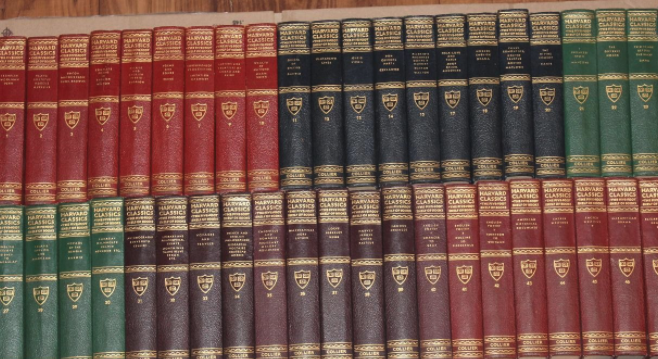
\includegraphics[width=4in]{books.png}
\end{figure}

\noindent He has 16 red books, 9 blue books, 7 green blooks and 10 purple books.

\benum
\subquestionwithpoints{4} If he randomly takes 4 books off the shelf \emph{with} replacement, what is the probability he gets all red books? \spc{3}

\subquestionwithpoints{4} If he randomly takes 4 books off the shelf \emph{without} replacement, what is the probability he gets all red books? \spc{3}

\subquestionwithpoints{4}  If he randomly takes 4 books off the shelf without replacement, what is the probability he gets two blue books and two purple books? \spc{3}

\subquestionwithpoints{5}  If he randomly takes 4 books off the shelf without replacement, what is the probability he gets two blue books then two purple books \emph{in that order}? \spc{4}

\subquestionwithpoints{4}  If he randomly takes 4 books off the shelf without replacement, what is the probability he gets books of all different colors? \spc{4}

\subquestionwithpoints{4}  If he randomly takes 4 books off the shelf without replacement, what is the probability he gets two books of one color and two books of a different color (e.g. two green books and two purple books)? This problem is hard, save it for last. \spc{4}

\subquestionwithpoints{3} He assigns each specific book to a specific student in his class to read. If he hands them out randomly, what is the probability at least one student will get their assigned book?\spc{1}

\eenum

\problem This problem is about the philosophical theory of probability.

\benum

\subquestionwithpoints{3} Experts at a think tank estimate war with North Korea at 50-50. What definition of probability was employed here? \spc{2}

\subquestionwithpoints{3} Pictured below is the \qu{bean machine}. A marble gets dropped in from the top and it makes its way down to a bin on the bottom. 

\begin{figure}[htp]
\centering
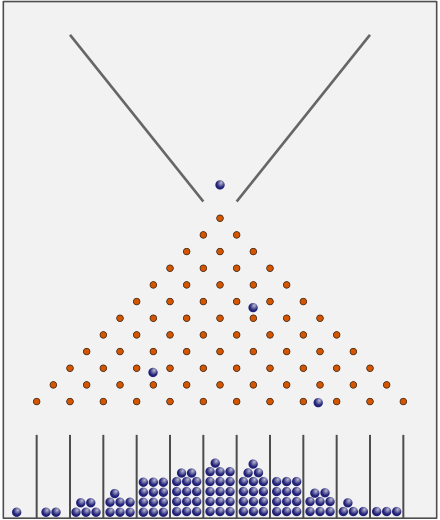
\includegraphics[width=3in]{bean.png}
\end{figure}

Only 0.8\% of the marbles wind up in the leftmost bin. What definition of probability was most likely employed to arrive at this number? \spc{2}

\subquestionwithpoints{3} If a marble was dropped down, would Laplace believe its final destination bin to be truly deterministic? Yes/no. \spc{2}


\eenum

\problem The incidence of cirrhosis in America is approximately 0.57\% but among alcoholics, it's 15\%. There are about 8 million alcoholics in America, a country with a total population of 323 million. Let the event $C$ denote cirrhosis and the event $A$ denote alcoholism.

\benum
\subquestionwithpoints{5} In a random sample of 12 Americans, what is the probability at least one of them is alcoholic? Compute and round to 3 significant digits. \spc{2}

\subquestionwithpoints{3} [Extra Credit] In a random sample of 86 Americans, what is the probability 59 of them are alcoholic? Compute and round to 3 significant digits. \spc{3}

\subquestionwithpoints{4} Find $\prob{AC}$. Compute and round to 3 significant digits. \spc{3}

\subquestionwithpoints{4} We do not know if Joe is an alcoholic or not. What is the best guess of the probability he develops cirrhosis? \spc{2}

\subquestionwithpoints{4} Prove or disprove: $A, C$ are independent events. \spc{4}

\subquestionwithpoints{4} Find the probability of not having cirrhosis and not being an alcoholic. Compute and round to 3 significant digits. \spc{4}

\subquestionwithpoints{8} Find the risk ratio of alcoholism in cirrhosis. Compute and round to 3 significant digits. Provide a one-sentence interpretation in English. \spc{2}


\eenum

\end{document}
%%%%%%%%%%%%%%%%%%%



\problem This problem is about the philsophical theory of probability.

\benum
\subquestionwithpoints{2} Let $p := \prob{\text{Trump wins the election in November}}$. Posit a \textit{numeric answer} for $p$. \spc{2}

\subquestionwithpoints{5} Explain why there is no \qu{correct} answer to (a). Make sure to mention in your answer which definition of probability you are invoking. \spc{2}

\subquestionwithpoints{2} Would Laplace believe that the event \qu{Trump wins the election in November} to be \emph{truly} random? Yes/no only. \spc{2}
\eenum


\problem This problem is about sets and the mathematical theory of probability.

\benum

\subquestionwithpoints{3}Simplify $\braces{\varnothing} \cap \braces{\braces{\varnothing}}$. \spc{0.5}

\subquestionwithpoints{3} Let $A = \braces{1,2,3}$ and $B = \braces{1,2,3,4}$. Simplify $2^A \cap 2^B$. \spc{0.5}

\subquestionwithpoints{3} Compute $\cprob{A}{A^C}$. \spc{0.5}

\subquestionwithpoints{6} Consider events $A$ and $B$. Prove that $\prob{A \cup B} \leq \prob{A} + \prob{B}$. Use the \qu{axioms} of the probability set function and your knowledge of set theory and \textit{any} theorems from class that may be useful. \spc{12}



\eenum

\problem For the most part, motor vehicles are produced with one of two types of transmissions: manual and automatic. Manual is less common in cities because it's considered more burdensome for drivers, especially in traffic.

\begin{figure}[htp]
\centering
\includegraphics[width=3in]{manualvsautomatic.jpg}
\end{figure}

The percentage of new manual vehicles produced for 2017 is 46.2\%. Americans consume 21.1\% of worldwide vehicles. And 6.5\% of new vehicles in American are estimated to be manual.

\benum
\subquestionwithpoints{2} Let $A$ denote the event that a new car is in America and $M$ denote the event that a new car has a manual transmission. What is $\prob{A}$? Compute explicitly. \spc{1}

\subquestionwithpoints{2} Let $A$ denote the event that a new car is in America and $M$ denote the event that a new car has a manual transmission. What is $\prob{M}$? Compute explicitly. \spc{1}


\subquestionwithpoints{2} Let $A$ denote the event that a new car is in America and $M$ denote the event that a new car has a manual transmission. What is $\cprob{M}{A}$? Compute explicitly. \spc{1}

\subquestionwithpoints{4} What is the probability that the car is in America given that it is a manual transmission? Compute explicitly. \spc{5}

\subquestionwithpoints{7} How much more likely is a car to be manual outside of America than within America? Compute explicitly. \spc{9}


\subquestionwithpoints{3} [Extra Credit] Odds Against an event $A$ is defined as $\prob{A^C} / \prob{A}$. What are the odds against a car being American given that its automatic? Compute explicitly. \spc{6}

\subquestionwithpoints{4} You see seven new cars go by in New York. What is the probability all of them were manual? Compute explicitly. \spc{4}

\subquestionwithpoints{6} You see seven new cars go by in New York. What is the probability at least one of them was manual? Compute explicitly. \spc{6}

\subquestionwithpoints{3} You see seven new \textit{manual} cars go by in New York. What is the probability the next one (the eigth car) is automatic? Compute explicitly. \spc{1}

\subquestionwithpoints{6} List all assumption(s) you use to answer (g), (h) and (i). There should be at least two. State if each assumptions is reasonable \textit{and why}.\spc{7}

\subquestionwithpoints{3} You go to a party with 20 cars and everyone puts their keys in a bag and the keys are distributed out randomly. What is the approximate probability at least one person gets the keys to their car? Compute approximately. \spc{2}


\eenum


\end{document}



\problem This question is about \qu{combination locks.} The particular model pictured below is called a MasterLock.

\begin{figure}[htp]
\centering
\includegraphics[width=3in]{masterlock.jpg}
\end{figure}

\noindent It has 40 notches labeled $\braces{0, 1, \ldots, 39}$. The lock is opened by entering the \qu{code} which consists of turning the lock to the right to the first number in the code, then turning one full rotation to the left and then to the second number in the code and finally turning right to the third number in the code. There are no restrictions on these three code numbers. Locks are identified by these three numbers and assume the locks are identical in every other way.

\benum
\subquestionwithpoints{3} Express $\Omega$, the universe of all possible lock combinations using set notation.\spc{2}

\subquestionwithpoints{3} How many unique locks can be produced? That is to say, how many codes are there? This is also $|\Omega|$.\spc{2}

\subquestionwithpoints{3} The locks are manufactured with the codes being equally likely. You go to the store and purchase one MasterLock. What is the probability the code is 21-10-32? No need to compute. \spc{2}

\subquestionwithpoints{3} The locks are manufactured with the codes being equally likely. Your friend goes to the store and purchases one MasterLock with the code 21-10-32. You also purchase a lock. What is the probability you get the same code? \spc{2}


\subquestionwithpoints{3} In one sentence, explain why the lock should not be called a \qu{combination lock} and instead be called a \qu{permutation lock.}\spc{2}

\subquestionwithpoints{3} In one sentence, explain why the lock should not be called a \qu{permutation lock} either.\spc{2}

\subquestionwithpoints{4} Assume that no numbers in the code are duplicated (each code number is unique and cannot be repeated). What is the probability of getting a lock where each number is less than 10 (that is 0, 1, \ldots, 9)? No need to compute explicitly.\spc{3}


\subquestionwithpoints{5} Assume that no numbers in the code are duplicated (each code number is unique and cannot be repeated). What is the probability of getting two even numbers and one odd number in the code (not necessarily in that order)? Note: zero is an even number; thus, there are twenty even numbers and twenty odd numbers in a MasterLock code number. \spc{3}


\subquestionwithpoints{4} What is the probability of getting a lock whose code consists of one odd number and two non-trivial powers of two i.e. from the set $\braces{2, 4, 8, 16, 32}$? \spc{2}


\eenum

\problem Imagine you are a contestant on the Monte Hall game. 

\begin{figure}[htp]
\centering
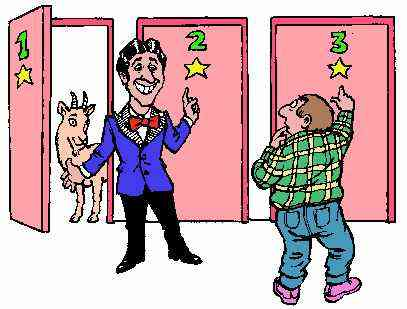
\includegraphics[width=2.3in]{montehall.jpg}
\end{figure}

Assume the same rules as we dicussed in class and that was on the homework. There are three doors with a hidden car in one and two smelly goats in the others. The location of the car is known by the gameshow host. You pick a door and the gameshow host opens a different door revealing one of the two goats. You now have the option to switch.

In this problem a similar situation as we talked about in class: assume the car is in door 2 but the contestant does not know thats.

\benum
\subquestionwithpoints{6} Draw the tree for this game with the following events: contestant first door pick (with states DP1, DP2, DP3), gameshow host door open (with states DO1, DO2, DO3), contestant win assuming contestant switches doors (with states W and L). Assume the car is in door 2. When drawing the tree, include all conditional probabilities and joint probabilities.\spc{10}

\subquestionwithpoints{5} Assuming the contestant has won, what is the probability the contestant chose door 1 as their first door pick?\spc{3}

\subquestionwithpoints{6} Assuming the host chose door 3 to open up, what is the probability the contestant won?\spc{3}


\subquestionwithpoints{5} Assume that if the contestant chose door 2 on the first pick, the game is repeated with 60\% probability but otherwise the normal rules of the game are in effect. What is the probability the contestant wins now?\spc{6}


\eenum

\problem This problem has theoretical questions that are not related to one another.

\benum

\subquestionwithpoints{3} What is the set of $\integers \backslash \rationals$?\spc{2}


\subquestionwithpoints{3} What is $\bigcup_{i=1}^{10} (-i,~i)$?\spc{1}

\subquestionwithpoints{4} Assume $\Omega = \braces{\omega_1, \omega_2, \omega_3}$ where each outcome is equally likely. Compute:

\beqn
\sum_{A \in 2^\Omega} \prob{A} = \hspace{400px}
\eeqn\spc{0.5}


\subquestionwithpoints{4} [Extra Credit] Repeat the calculation in the previous question except with $\Omega$ now having an arbitrary number of outcomes, $n$. Answer as succinctly as possible (use the most compact notation). \spc{4}


\subquestionwithpoints{5} Assume that $\prob{A} > 0$ if $A$ is non-empty. If $A \subset D$, prove that $\prob{A} < \prob{D}$. Prove it from the definition of probability as well as what you know from set theory.\spc{9}


\subquestionwithpoints{4} Using all theorems and facts from class, prove that:

\beqn
\prob{A^C \cap B^C} = 1 - \prob{A} - \prob{B} + \prob{A \cap B}
\eeqn\spc{4}


\subquestionwithpoints{3} In the multinomial expansion of $(a+b+c+d+e+f)^{600}$, how many terms are $a^{100} b^{100} c^{100} d^{100}e^{100}f^{100}$? No need to compute explicitly.\spc{2}


\subquestionwithpoints{4}  Approximate 1000! as 10 to the power of some number. Compute that number to one decimal place.\spc{3}

\subquestionwithpoints{3}  If $a = \binom{999}{500}$ and $b = \binom{999}{499}$, express $\binom{1000}{500}$ as a function of $a$ and $b$.\spc{2}


\subquestionwithpoints{3} What is the probability that OJ Simpson was guilty of the homicides he was accused of?\spc{2}


\subquestionwithpoints{4} Why is the long run frequency definition of probability not adequate to define the probability you came up with in the previous question? \spc{3}

\subquestionwithpoints{3} Laplace believed in universal determinism. If he thought everything was predetermined, how would he explain how a coin flips randomly to heads or tails? \spc{5}

%\subquestionwithpoints{3} Explain using estimates of conditional and unconditional probabilities why the events \qu{having lung cancer} (denoted by B) and \qu{being a smoker} (denoted by A) are independent or dependent. Use the same reasoning we used in class. \spc{3}

\subquestionwithpoints{4} A company has 20 trucks and 10 grocery stores. If each truck carries the same load (i.e. they can be considered indistinct) but each grocery store is different, how many ways is there to send the 20 trucks to the 10 grocery stores such that each store gets at least one shipment? No need to compute explicitly. \spc{3}

\subquestionwithpoints{4} 20 couples enter a ballroom. Each man chooses a random girl to dance with. What is the approximate probability no man dances with his girlfriend?
\eenum




\end{document}
